\subsection{Histogram computation}\label{sec:histogram}

The computation of a histogram is one of the most common tasks in data analysis. A histogram
succinctly summarizes the distribution of sample values, and thus is useful as a cursory ``look''
into the data and in guiding further analysis. For example, it can be used to guide the selection of
colors and opacities in transfer functions.

We choose Intersection~\cite{histogram_intersection1991} as the metric of choice, because it is fast
to compute and is reasonably insensitive to changes in precision, as well as the number of bins. The
intersection distance between two histograms $H_1$ and $H_2$ is defined as
$e(H_1,H_2)=\sum_{i}{\min{(H_1(i),H_2(i))}}$ (the sum is over all bins $i$). Every histogram is
normalized by dividing each bin by the total number of samples in the volume. Our error metric takes
into account not only the shapes but also the value ranges of the histograms. Therefore, when
computing the histogram of a reconstructed function, we clamp its range of values to that of the
original function, so that corresponding histogram bins, i.e., $H_1(i)$ and $H_2(i)$, share the same
range.

As before, for each data set, we use~\Cref{alg:greedy} to compute an \shop stream, optimized for
histogram error, and an \shsg from its signature. We plot the error curves for all relevant
streams using the error metric just defined~(compare \Cref{fig:histogram-stream-comparison}). We use
64 for the number of bins, but note that there exist no meaningful differences across a wide range
of number of bins (from 64 to 512) in our experiments. In all cases, the group consisting of
\sbit, \slvl, and \smag underperforms the other group by a large margin.

Among the former group, \slvl generally outperforms \sbit at low bit rates, although there are
several crossover points between the two curves. These crossover points are explained
in~\Cref{fig:histogram-explain}. When leading zero packets are present, \slvl outperforms
\sbit, because increasing resolution does not help produce an accurate histogram as much as
increasing precision. The histogram is oblivious to spatial locations of samples (which require
resolution to resolve), but it is sensitive to sample values (which require precision). However,
when leading zero packets are removed, as is the case when using compression, \sbit benefits
significantly more than \slvl does (for the same reason explained in~\Cref{sec:rmse-optimized}),
resulting in the observed crossovers. Finally, \smag performs poorly, because it ignores regions
of smooth variations, which nevertheless count toward the distribution.

In the other group, the performances of \swav and \shsg (and even \shop) differ by negligible
amount. This observation is confirmed in~\Cref{fig:histograms-boiler}, where we plot various
histograms, reconstructed at 0.13 bps, for the \emph{boiler} data set. The histograms produced by
\swav and \shsg have approximately the same shape, and are the closest to the reference histogram.
The next best histogram is produced by \slvl, followed by the one produced by \sbit, and finally
\smag. These results suggest that histogram computation is among the analysis tasks that benefit
significantly from a bit ordering that combines both resolution and precision, not one that adheres
to either exclusively.

\begin{figure*}[h]
	\centering
	\subcaptionbox{\emph{boiler}}
	{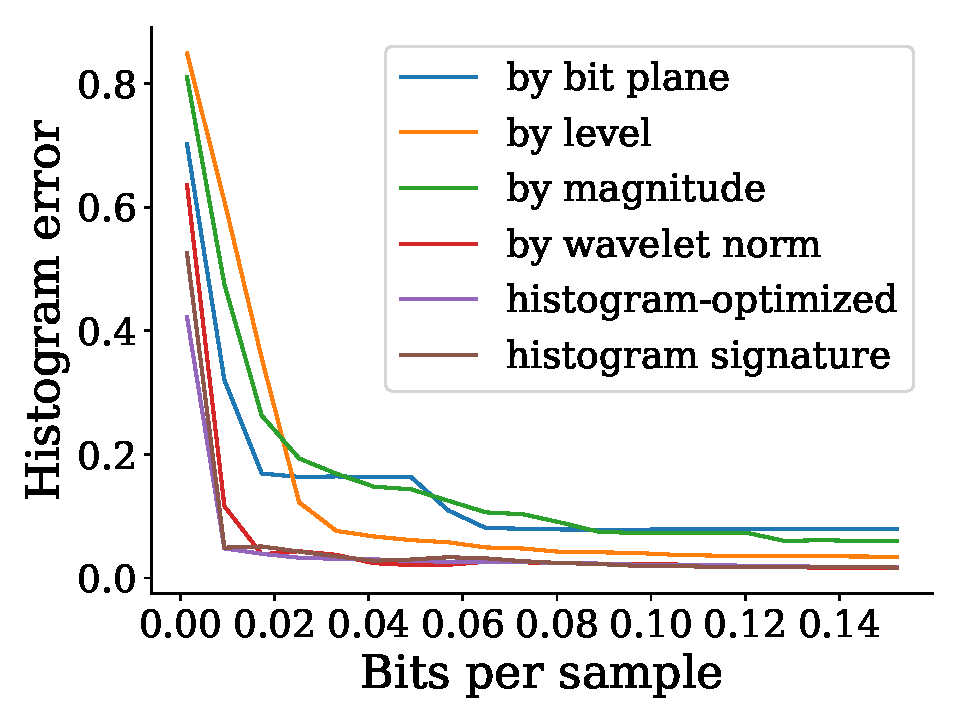
\includegraphics[width=0.24\linewidth]{histogram/histogram-optimized-boiler}}
	\subcaptionbox{\emph{diffusivity}}
	{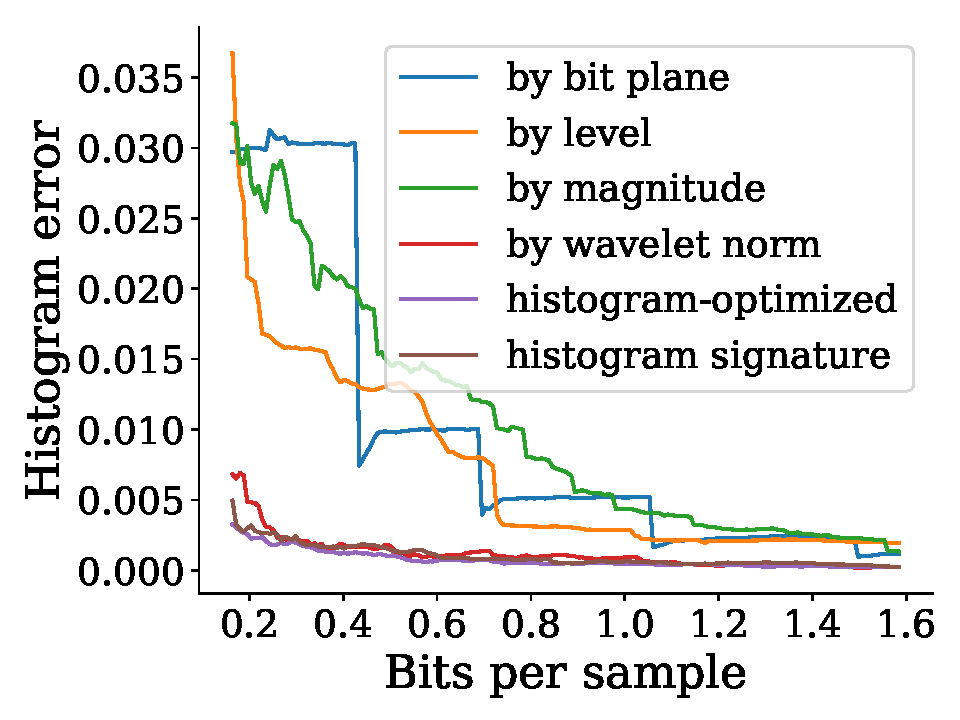
\includegraphics[width=0.24\linewidth]{histogram/histogram-optimized-diffusivity}}
	\subcaptionbox{\emph{kingsnake}}
	{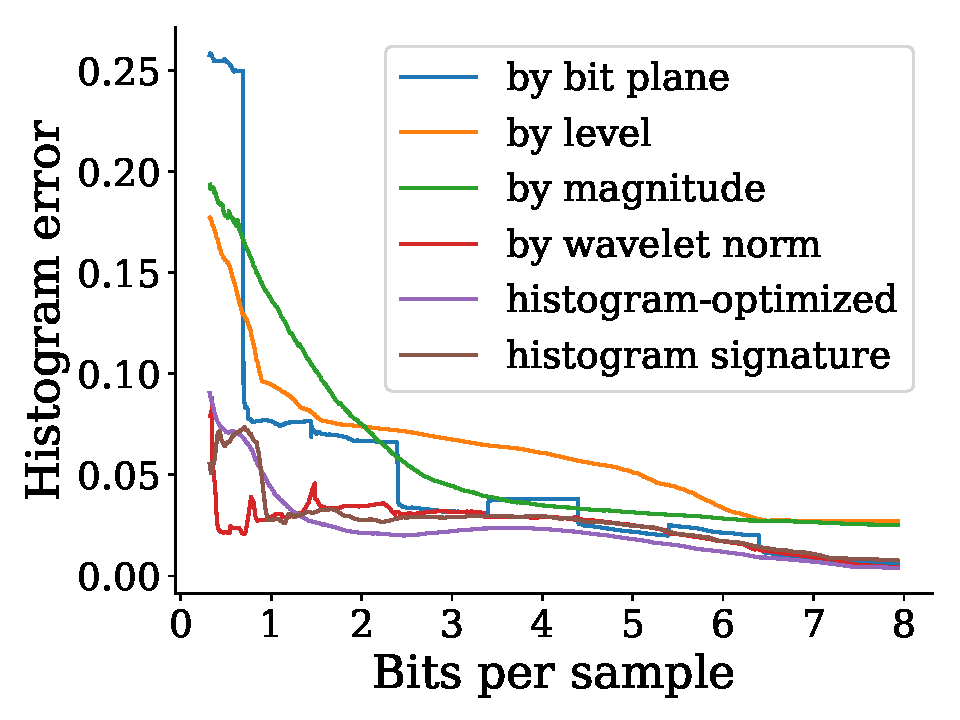
\includegraphics[width=0.24\linewidth]{histogram/histogram-optimized-kingsnake}}
	\subcaptionbox{\emph{foam}}
	{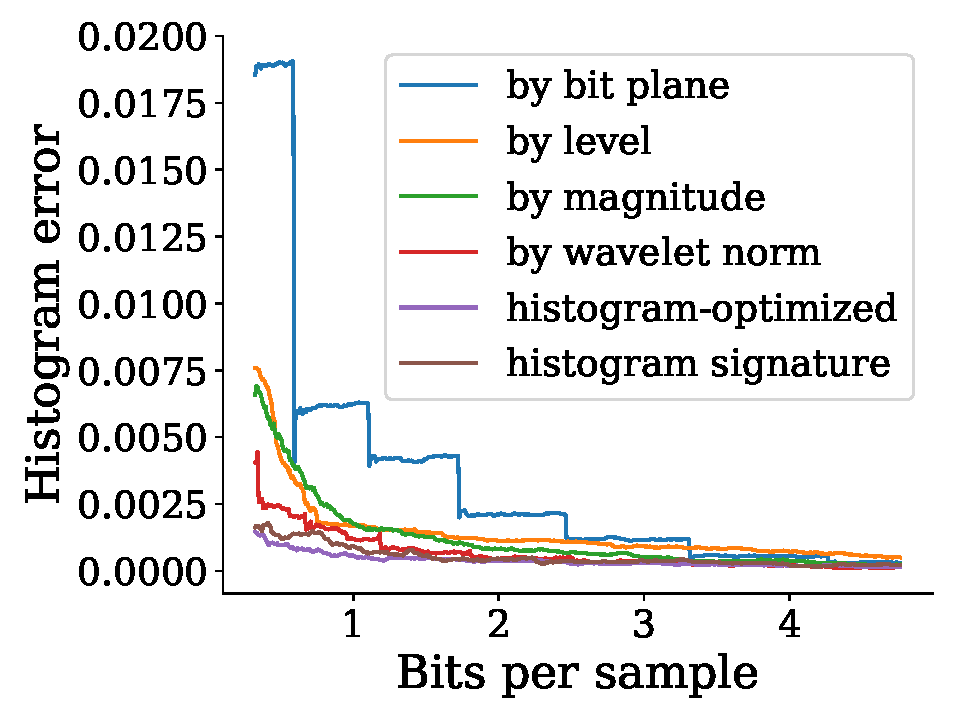
\includegraphics[width=0.24\linewidth]{histogram/histogram-optimized-foam}}
	\caption{Comparison of histogram errors among streams. Plots are truncated to highlight
	differences without hiding important trends. In general, in terms of error, $\shop \approx
	\shsg \approx \swav < \slvl < \sbit < \smag$. Crossover points between \sbit and \slvl are
	explained in~\Cref{fig:histogram-explain}}.
	\label{fig:histogram-stream-comparison}
\vspace{1em}

	\centering
	\subcaptionbox{\emph{by level} (\slvl)}{
	{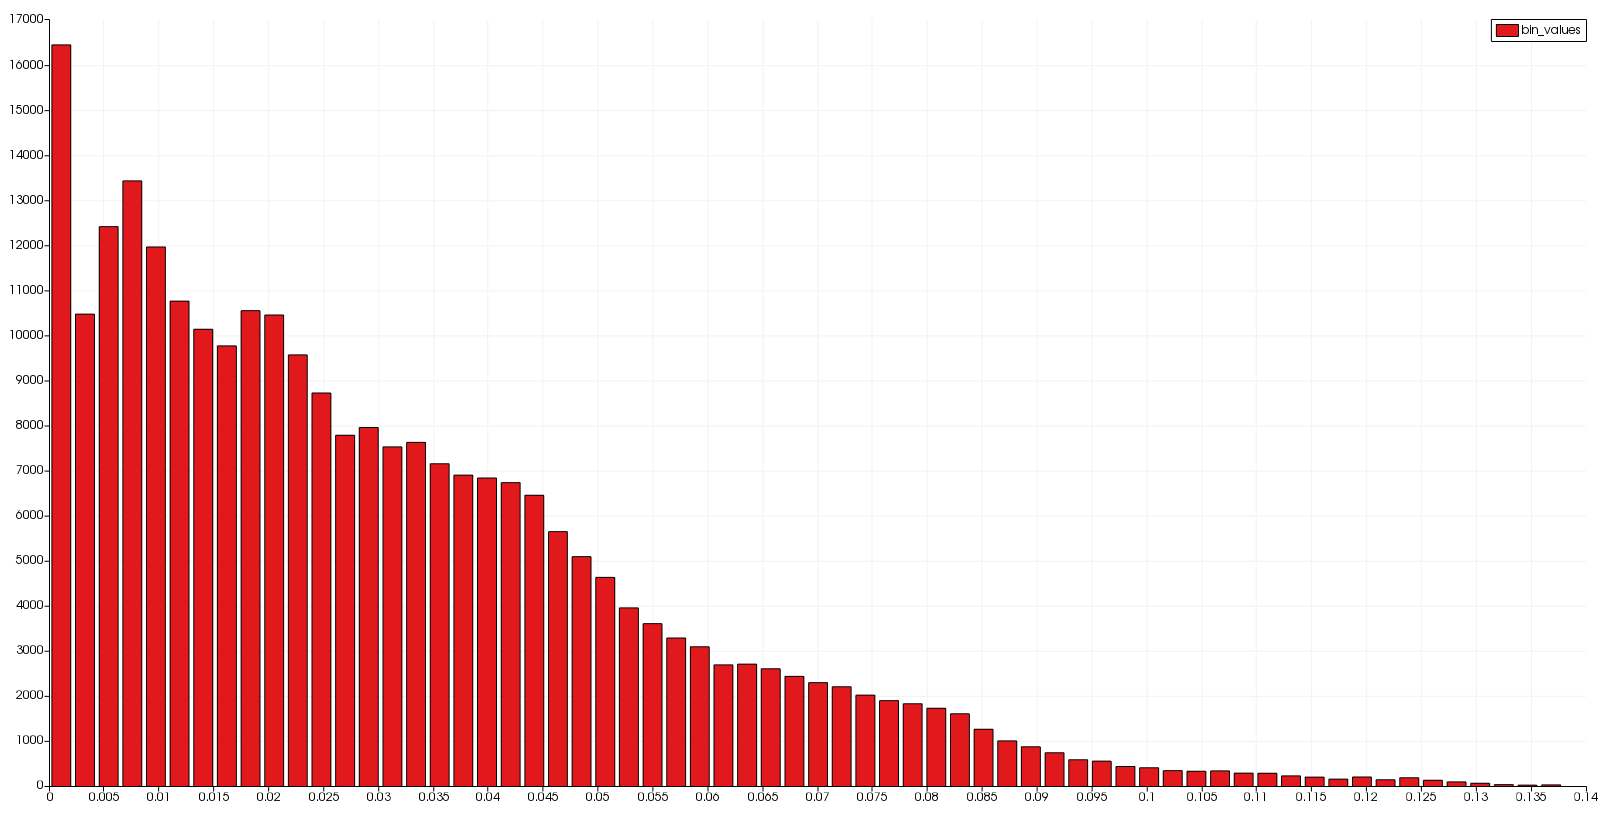
\includegraphics[width=0.155\linewidth]{histogram/histogram-boiler-level.png}}}
	\subcaptionbox{\emph{by bit plane} (\sbit)}{
	{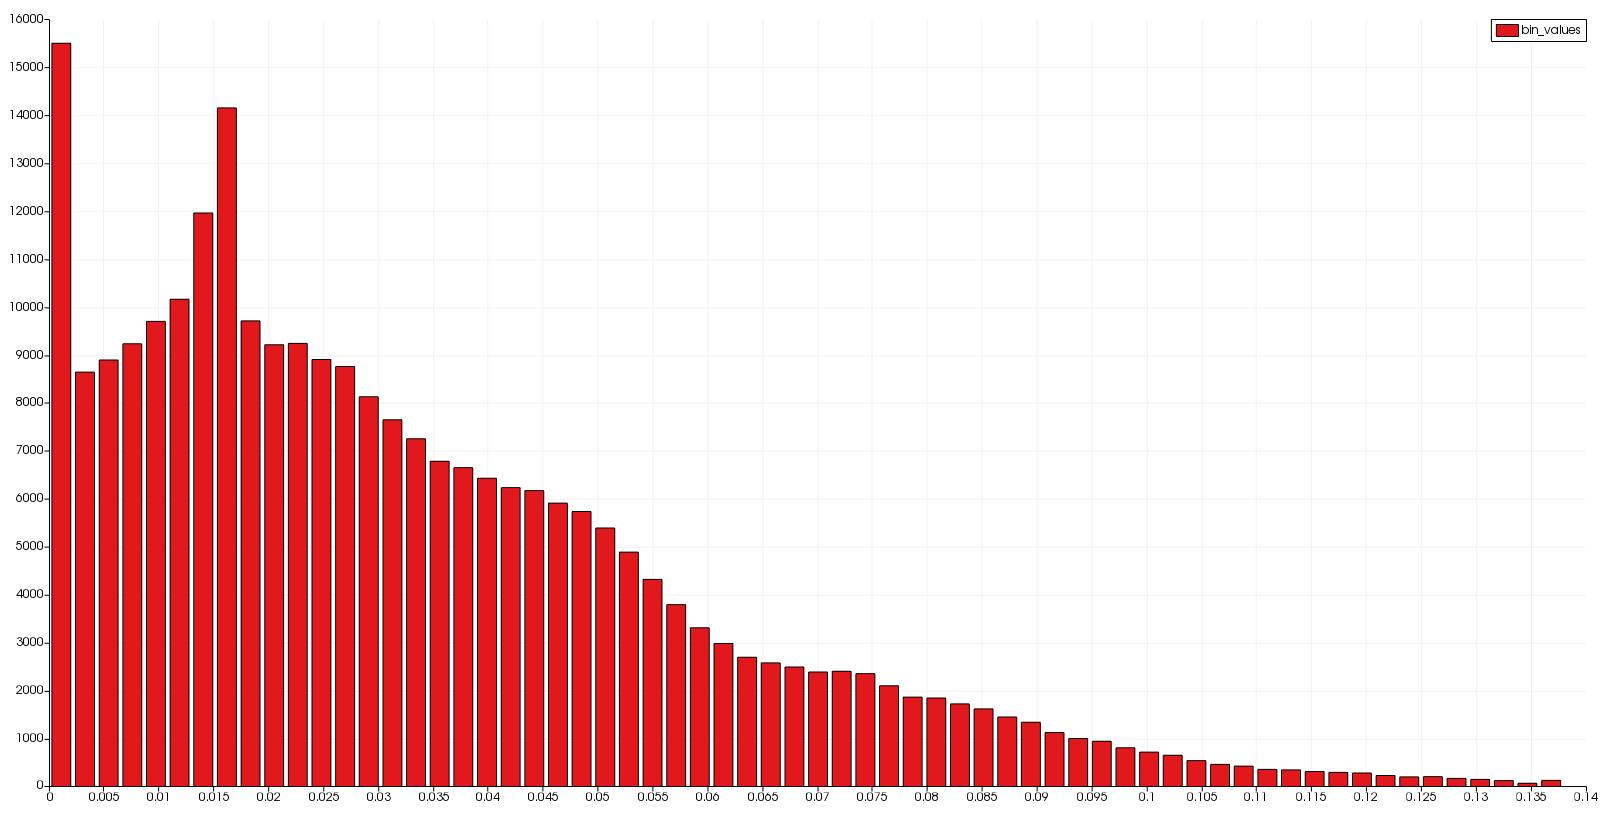
\includegraphics[width=0.155\linewidth]{histogram/histogram-boiler-bit-plane.png}}}
	\subcaptionbox{\emph{by magnitude} (\smag)}{
	{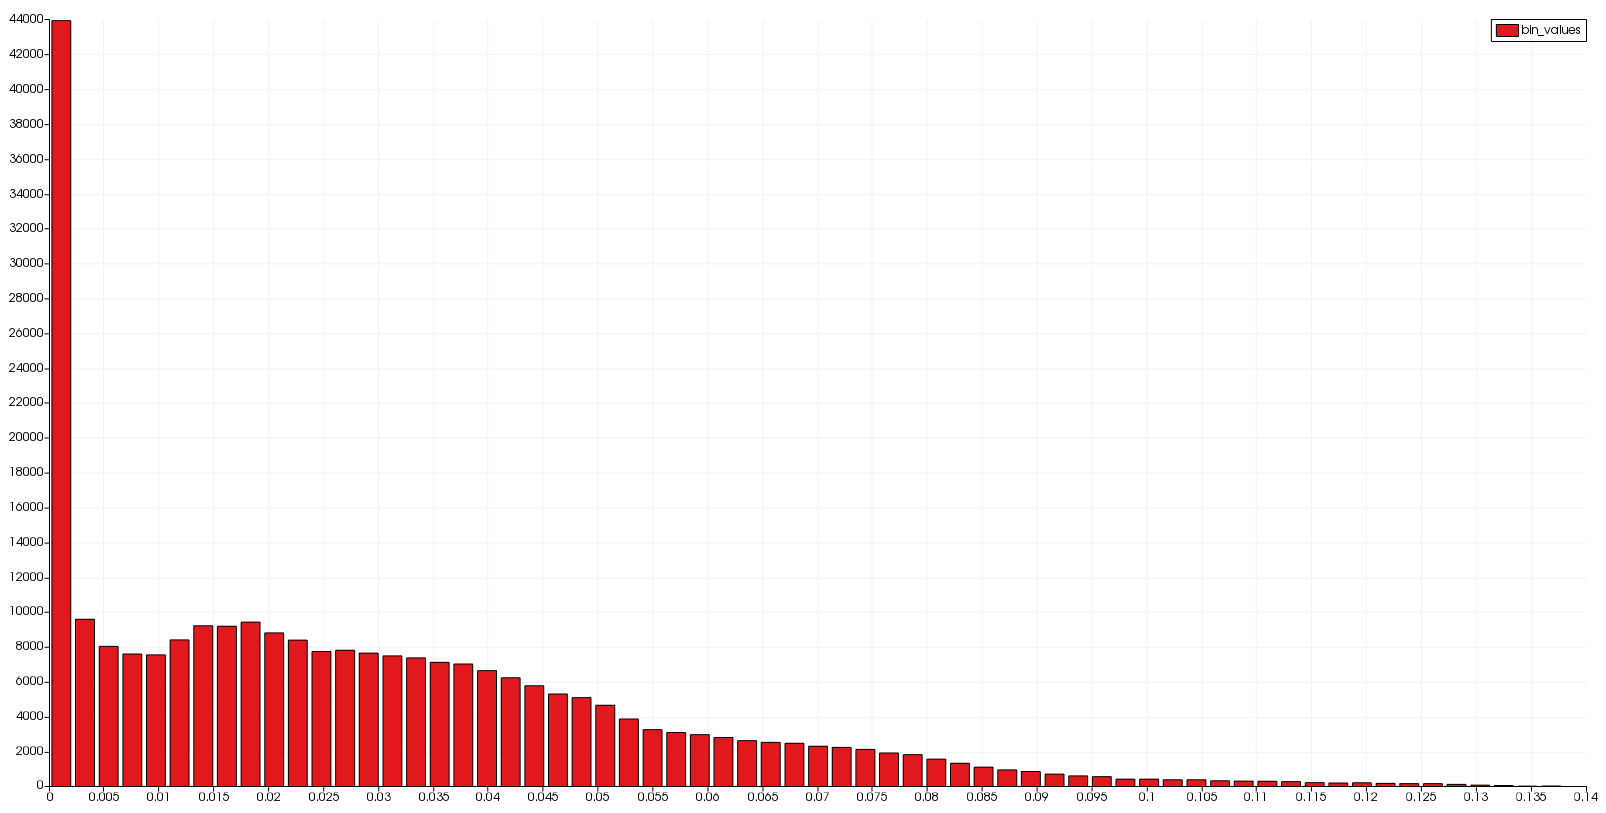
\includegraphics[width=0.155\linewidth]{histogram/histogram-boiler-magnitude.png}}}
	\subcaptionbox{\emph{by wavelet norm} (\swav)}{
	{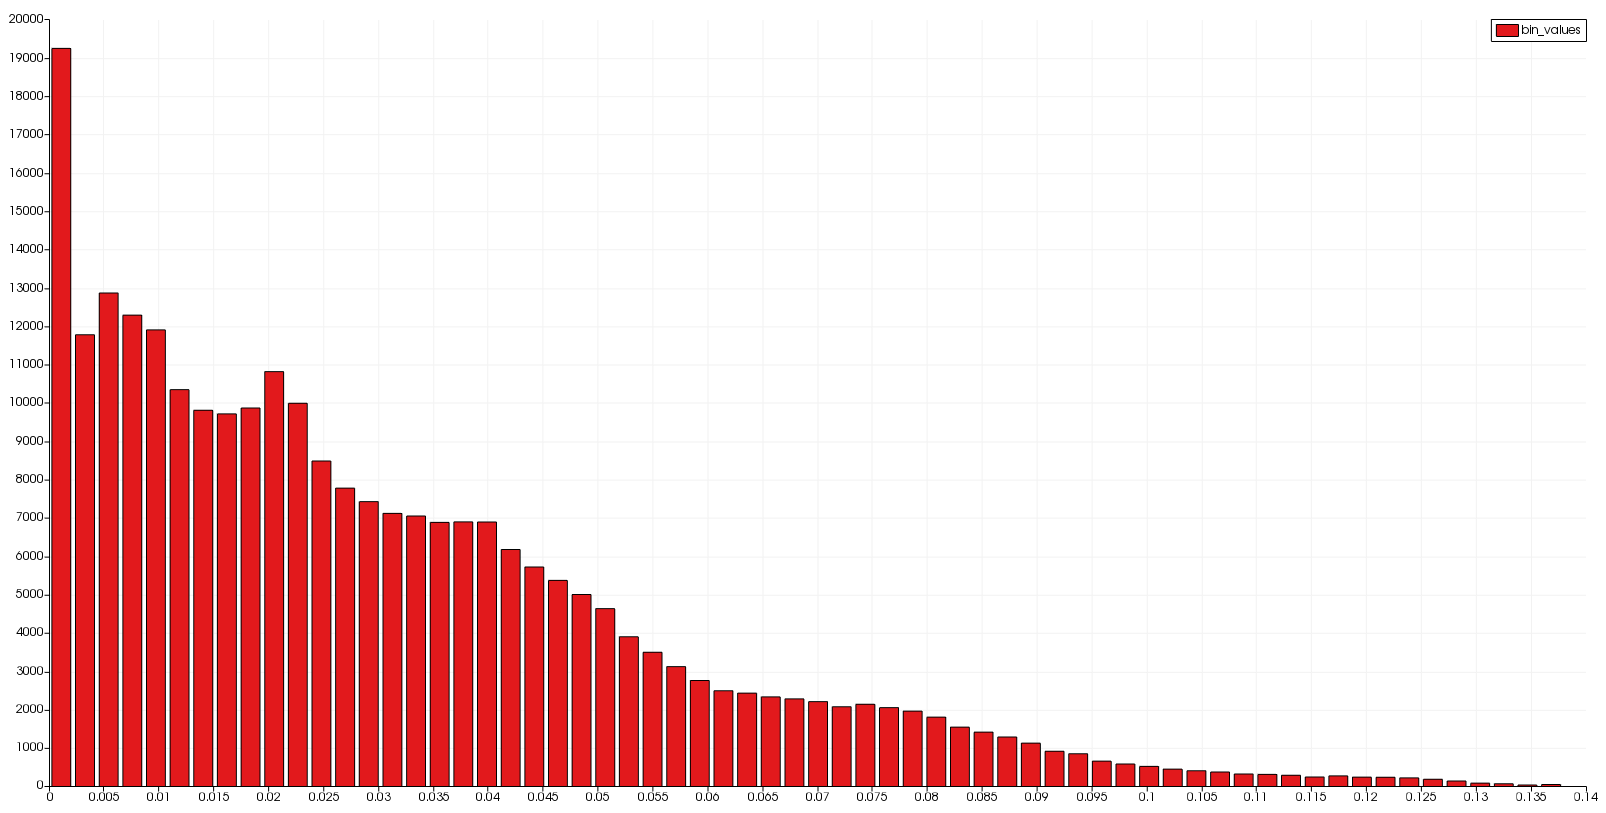
\includegraphics[width=0.155\linewidth]{histogram/histogram-boiler-wavelet-norm.png}}}
	\subcaptionbox{\emph{by signature} (\shsg)}{
	{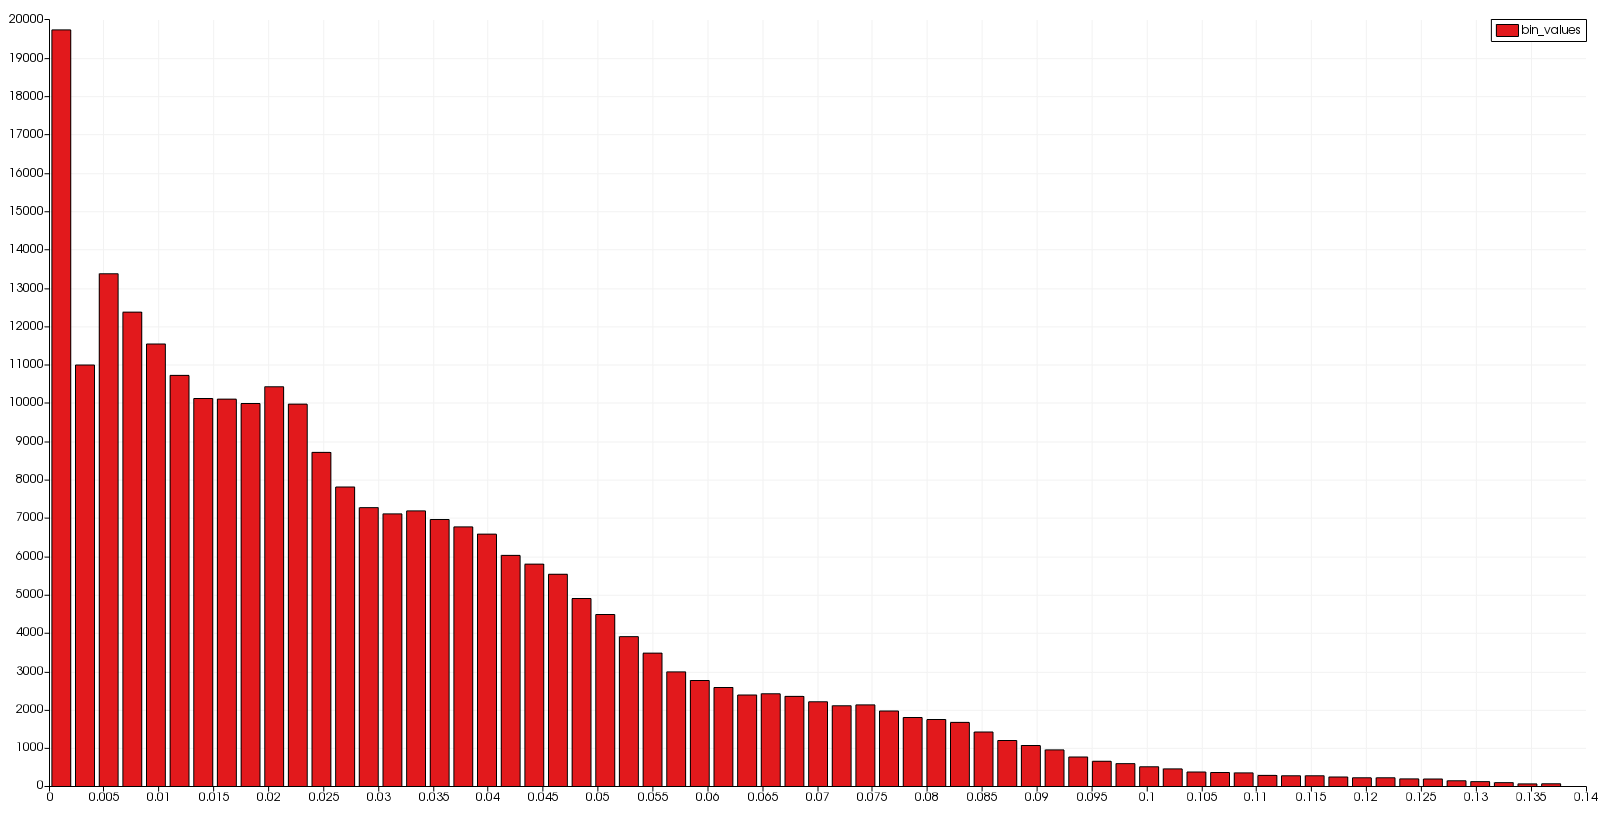
\includegraphics[width=0.155\linewidth]{histogram/histogram-boiler-signature.png}}}
	\subcaptionbox{\emph{reference}}{
	{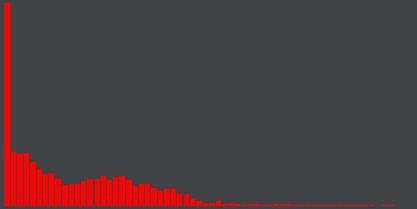
\includegraphics[width=0.155\linewidth]{histogram/histogram-boiler-groundtruth.png}}}
	\caption{Histograms of the \emph{boiler} data set, reconstructed at 0.13 bps. \slvl, \swav, and
	\shsg produce histograms that share a shape similar to the reference histogram, with most of the
	peaks and valleys preserved. In contrast, \sbit produces a spurious peak not found in the
	reference. Finally, \smag's histogram has a widely skewed distribution where too many values fall
	into the first bin.}
	\label{fig:histograms-boiler}
\end{figure*}

\begin{figure}[h]
	\centering
	\subcaptionbox{with leading zero packets}
	{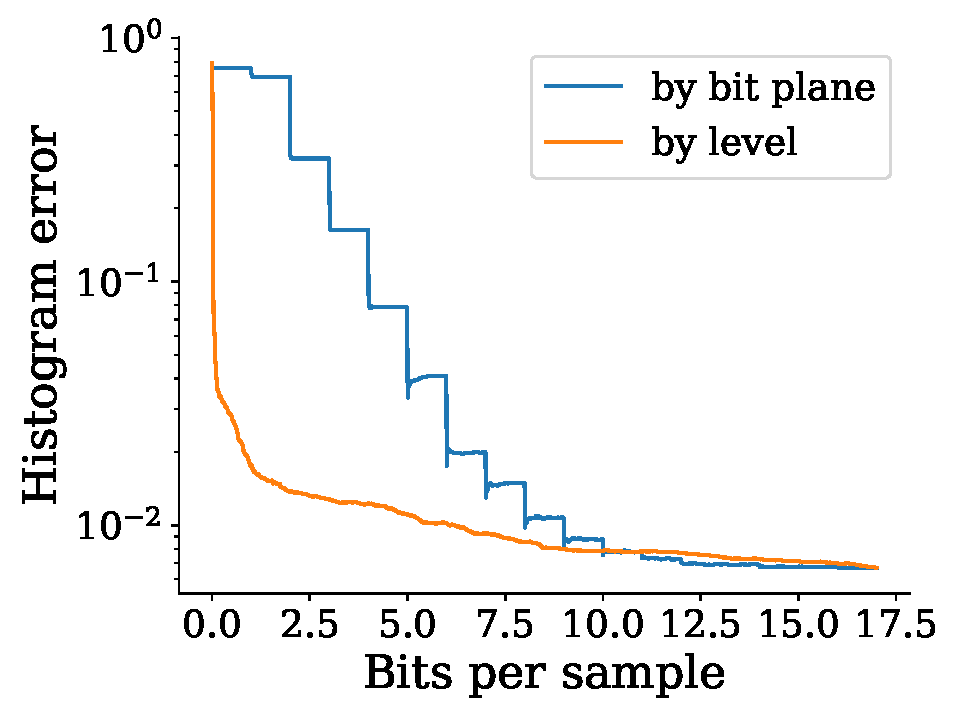
\includegraphics[width=0.48\linewidth]{histogram/histogram-explain-boiler-wlz}}
	\subcaptionbox{without leading zero packets}
	{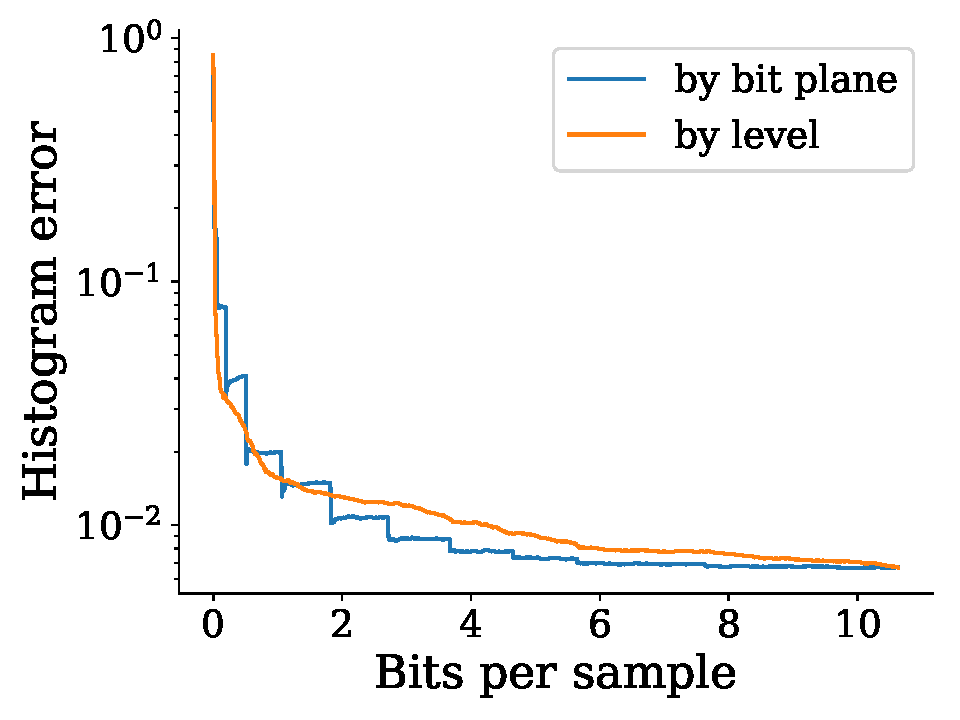
\includegraphics[width=0.48\linewidth]{histogram/histogram-explain-boiler}}
	
	\caption{Comparison of histogram error curves produced by \sbit and \slvl, for \emph{boiler}, with
	and without leading zero bits. The vertical axis is in log scale. The error for \sbit reduces in a
	stair-step fashion, in which each step corresponds to a new bit plane streamed. \sbit benefits
	significantly more from the removal of leading zero bits (from (a) to (b), the blue curve shifts
	more to the left).}
	\label{fig:histogram-explain}
\end{figure}
